\documentclass[a4paper,12pt]{article}
\usepackage[a4paper, left=2.5cm, top=2.5cm, right=2.5cm]{geometry}
\usepackage{amsmath, amssymb}
\usepackage{graphicx}
\usepackage{float}
\usepackage{booktabs}
\usepackage{hyperref}
\usepackage{setspace}
\usepackage{geometry}
\usepackage{natbib}

\geometry{
    left=1in,
    right=1in,
    top=1in,
    bottom=1in,
}

\begin{document}

\begin{titlepage}
    \centering
    \vspace*{2cm}
    
    {\Large \textbf{ATS Mandatory Assignment 05}}\\[1.5cm]
    
    {\large Mat-Nr: \\ 601223 \\ 6940188 \\[0.5cm]
    Universität Tübingen}\\[1cm]
    
    {\large Date of Submission: January 12, 2025}\\[1.5cm]
    
    \vfill
\end{titlepage}

\pagenumbering{gobble}
\newpage
\tableofcontents
\newpage

\pagenumbering{arabic}
\setcounter{page}{1}

\section{Introduction}
Time series data arise in numerous domains, ranging from economics and finance to engineering and machine learning. To analyze and forecast such data, models must capture both persistence (via autoregressive terms) and short-term shocks (via moving-average terms). Autoregressive Moving Average (ARMA) models are a common choice for this purpose, striking a balance between flexibility and interpretability.

In practice, analysts often observe only a single realization of the underlying stochastic process. This limitation necessitates using statistical properties such as stationarity, which ensures that the mean and variance of the series remain constant over time. Once stationarity is established, the subsequent challenge is parameter estimation. Maximum Likelihood (ML) estimation provides a rigorous framework for this task, offering desirable properties like consistency and efficiency, assuming the correct likelihood is specified. Yet, in many real-world settings, the true distribution of the innovations may be unknown or difficult to specify. Quasi-maximum likelihood estimation (QMLE) can then serve as an alternative, delivering robust estimates even when the likelihood is misspecified.

This paper focuses on an ARMA(1,1) model with heavy-tailed \(t\)-innovations. We investigate how two estimation strategies, Conditional Maximum Likelihood (CML) and Quasi-Maximum Likelihood (QML), perform under both correctly specified and misspecified likelihoods. First, we will verify the stationarity of our simulated data via a Dickey-Fuller test (Section~\ref{unitroot}). Next, we will estimate model parameters under each scenario, and finally, examine how sample size, confidence intervals, and heavy tails interact to influence the reliability of our inferences.

\section{Data Generating Process}
To demonstrate these ideas, we simulate data from an ARMA(1,1) model, whose details appear in Equation~\ref{eq:arma}. The model features an autoregressive parameter \(\phi\) and a moving-average parameter \(\theta\), with heavy-tailed \(t\)-innovations (\(\epsilon_t\)) of four degrees of freedom. Since \(\lvert \phi \rvert < 1\), the process is stationary in theory, implying a constant mean and variance.

We generate \(T = 800\) observations and discard the first 50 as a burn-in phase to mitigate dependence on arbitrary starting values. These initial values are set to the theoretical mean, \(\mu\), given in Equation~\ref{eq:Mean}. A plot of the simulated data (Figure~\ref{fig:simulated_arma}) exhibits fluctuations around \(\mu\), along with occasional outliers arising from the heavy-tailed error distribution. The autoregressive term introduces persistence between consecutive observations, whereas the moving-average component adds short-term random variation.

Although our ARMA(1,1) specification ensures \(\lvert \phi \rvert < 1\), we must still confirm stationarity from the single realization we observe. Therefore, we proceed by testing for a unit root, as described next.

\section{Unit Root Testing}
\label{unitroot}
Stationarity is vital for applying results like the law of large numbers and for enabling consistent parameter estimation. To this end, we employ the Dickey-Fuller (DF) test, which evaluates the presence of a unit root. The null hypothesis posits \(\rho = 1\) (non-stationarity), while the alternative suggests \(\rho \neq 1\).

Before implementing the test, we revisit Figure~\ref{fig:simulated_arma}, which shows our ARMA(1,1) series fluctuating around a nonzero mean of 40. This prompts us to choose **Case 2** of the DF test (an intercept but no trend), since assuming a zero-mean process (Case 1) would reduce test power, and Cases 3 or 4, permitting drift or trend, do not match the observed data. We then estimate the model (Equation~\ref{eq:alternative}) under the null hypothesis \(\rho = 1\) and the alternative \(\rho \neq 1\) via Ordinary Least Squares (OLS), obtaining \(\hat{\rho} = 0.96\) and \(\hat{\alpha} = 1.46\), with respective standard errors of 0.01 and 0.4. Notably, \(\hat{\rho}\) is close to the theoretical \(\phi\) value, while \(\hat{\alpha}\) deviates more, reflecting a higher standard error.

Next, we compute the DF statistic (Equation~\ref{eq:dftstat2}) and compare the result with Dickey-Fuller critical values. With over 500 observations and no trend at the 5\% significance level, the critical value is approximately \(-2.86\). Our test statistic of \(-3.66\) is below this threshold, leading us to reject \(H_0\) and conclude that the process is stationary.

Having verified stationarity empirically (via the DF test), we proceed to estimate the ARMA(1,1) parameters using Maximum Likelihood (ML). In the following section, we will initially assume the correct density for the innovations and later examine how misspecifying that density affects parameter estimates and inference.

\section{Maximum Likelihood Estimation}
For the parameter estimation, we will now employ Maximum Likelihood estimation, specifically Conditional Maximum Likelihood (CML). Unlike exact Maximum Likelihood, CML treats the first observation, \(y_1\), as deterministic and maximizes the likelihood conditioned on this value \citep[pp.~122--123]{Hamilton1994}. This approach is computationally efficient, and for a sufficiently large sample, the first observation contributes negligibly to the overall likelihood. Furthermore, given the stationarity condition \(\lvert \phi \rvert < 1\) (as established earlier), both Maximum Likelihood Estimators (MLE) and Conditional MLE share the same large-sample distribution.

To obtain the maximum likelihood estimates, we follow two steps. First, we propose two distinct parameter specifications and compare their respective log-likelihood values. This comparison indicates which specification better fits the data, offering insights into the process dynamics. Next, we estimate the parameters via a numerical search, effectively minimizing the log-likelihood.

\subsection{Estimating the Likelihood}
To implement our first approach, we compute the conditional log-likelihood contributions at each time step, thus requiring us to specify the densities for each observation. Assuming correct specification of the densities (i.e., knowing that the process innovations follow a \(t\)-distribution), the conditional log-likelihood for each observation is given by Equation~\ref{eq:cml}. Working with the logarithm of these densities, rather than the densities themselves, enables us to sum the log-densities rather than multiply them, thereby improving numerical stability (Equation~\ref{eq:ll}).

The total conditional log-likelihood is obtained by summing these contributions over all time steps (Equation~\ref{eq:tcl}). In the following analysis, we use two parameter specifications to compute the conditional log-likelihood. First, we calculate it for the true parameters that generated the series. We then compare this value to the log-likelihood obtained using an alternative specification. These two parameter sets are given in Section~\ref{specifica}, and the corresponding results are presented in Table~\ref{tab:log_likelihood_results}.

The results show that the conditional log-likelihood for Case (a) (the true parameter specification) is notably higher (less negative) than that for Case (b), indicating that the true parameters better capture the observed series. In log-likelihood terms, higher (or less negative) values imply a greater probability density for the data, suggesting that the specified parameters are more likely to have generated the series. In contrast, deviations in the AR and MA coefficients, as well as in the degrees of freedom \(\nu\), result in a less accurate representation of the data-generating process.

This discrepancy underscores CMLE’s sensitivity to parameter specification. By explicitly modeling heavy-tailed \(t\)-distributed innovations, CMLE effectively differentiates among parameter sets, favoring those closely aligned with the actual data-generating mechanism.

\subsection{Parameter Estimation via Numerical Minimization}
To estimate the parameters \( c, \phi, \theta, \nu \), we minimize the negative log-likelihood rather than directly maximizing the log-likelihood. This transformation, multiplying the log-likelihood by \(-1\), is mathematically equivalent to maximizing the original function, since multiplying by \(-1\) does not change the location of the optimum. We modify the log-likelihood from Equation~\ref{eq:tcl} to return its negative value, thus making it compatible with standard optimization routines designed to find a minimum.

We employ MATLAB’s \texttt{fminsearch} (a derivative-free method) to carry out this minimization and specify a Hessian-based covariance matrix to quantify parameter uncertainty. As initial guesses, we use \(c = 1.5\), \(\phi = 0.75\), \(\theta = 0.5\), and \(\nu = 5\). The results of this optimization appear in Table~\ref{tab:optimization_results} and indicate that the Conditional Maximum Likelihood Estimation (CMLE) approach successfully recovers the ARMA(1,1) parameters. The estimated values for \(c\), \(\phi\), \(\theta\), and \(\nu\) all closely match their true values, thereby confirming the accuracy of the method. For instance, \(\hat{c} = 2.2456\) is near the true \(c = 2\), \(\hat{\phi} = 0.9446\) approximates the true \(\phi = 0.95\), \(\hat{\theta} = 0.2834\) aligns with the true \(\theta = 0.25\), and \(\hat{\nu} = 3.4515\) effectively captures the heavy-tailed nature of the process (\(\nu = 4\)).

Standard errors derived from the Hessian-based covariance matrix are relatively small, reflecting reasonable precision for all parameter estimates. Notably, the minimized negative log-likelihood of \(1386.5\) suggests a good fit to this specific realization, even slightly improving upon the true parameters’ log-likelihood value of \(-1388.32\). This outcome may arise because the optimization tailors estimates to the observed data, compensating for random fluctuations in the finite sample.

\subsection{Confidence Intervals}
To further assess the precision of the estimates, we construct 95\% confidence intervals. These intervals indicate the range within which the true parameter values are likely to lie, given the data. In particular, if the true parameter value falls within the interval, we fail to reject the null hypothesis (at the 5\% level) that this value matches our estimate.

Since the asymptotic distribution of Maximum Likelihood estimators is normal, we rely on the usual normal quantiles for constructing the 95\% intervals. Table~\ref{tab:firstconfidence_intervals} presents these results. All estimates lie within their respective intervals, implying that we cannot reject the hypothesis that our estimates equal the true values at a 5\% significance level. However, the intervals—especially for \(c\) and \(\nu\)—are comparatively wide, indicating greater uncertainty for these parameters. Overall, the findings underline the statistical significance of our estimates and demonstrate the consistency property of Maximum Likelihood estimation.

\subsection{T-test}
Building on the confidence-interval insights, we now turn to hypothesis testing by examining whether the autoregressive coefficient \(\phi\) significantly differs from 0.8. We use a \(t\)-test at a 5\% significance level, evaluating whether the data provide sufficient evidence to reject the hypothesized value of \(\phi = 0.8\). As shown in Equation~\ref{eq:nullacht}, the null hypothesis posits \(\phi = 0.8\), while the alternative states \(\phi \neq 0.8\). The corresponding test statistic is defined in Equation~\ref{eq:tstatmlone}.

Under the large-sample asymptotic normality of the MLE, we adopt the conventional critical value of \(1.96\) at the 5\% level. Our calculated statistic, \(t = 14.52\), substantially exceeds \(1.96\), leading us to reject \(H_0: \phi = 0.8\) at the 5\% significance level. This conclusion is further supported by the two-sided \(p\)-value, which indicates the probability of observing a test statistic as large as \(14.52\) under \(H_0\). Since \(p < 0.05\), we reject the null hypothesis that \(\phi\) equals 0.8 with 95\% confidence.

\subsection{Increasing the Sample Size}
To explore key properties of Maximum Likelihood Estimators (MLE), including efficiency, consistency, and asymptotic normality, we first increase the sample size from 800 to 50{,}000 observations. We then adopt a less conventional approach of performing repeated simulations with a fixed sample size, providing insights into the distribution of parameter estimates across different realizations of the process.

By re-estimating the parameters via Conditional Maximum Likelihood (CML), constructing confidence intervals, and conducting hypothesis tests, we assess how a larger sample affects the precision of estimates, the outcomes of hypothesis tests, and the covariance matrix computation. Table~\ref{tab:optimization_large_sample} summarizes the parameter estimates for \(T=50{,}000\) observations, obtained by minimizing the negative log-likelihood (using the same initial values as before).

The results confirm that increasing the sample size enhances both the accuracy and the precision of the estimates: all four parameters now lie closer to their true values. Table~\ref{tab:confidence_intervals_large_sample} shows that standard errors decrease substantially, reflecting improved precision. For instance, the standard error of \(c\) drops from 0.40 to 0.05, and the covariance matrix also shows smaller elements, indicating reduced uncertainty as \(T\) grows.

Meanwhile, the negative log-likelihood rises from 1386.5 (at \(T=800\)) to 84{,}302 (at \(T=50{,}000\)), a predictable outcome because the log-likelihood increases with the number of observations. The 95\% confidence intervals likewise narrow, highlighting enhanced parameter stability. Moreover, all estimates again lie within their respective intervals, so we do not reject the hypothesis that these estimates match the true values at the 5\% level.

If we return to the null hypothesis from Equation~\ref{eq:nullacht} (\(\phi=0.8\)) and switch to the test statistic in Equation~\ref{eq:tstatmltwo}, we again use the critical value of 1.96 (assuming asymptotic normality). Because the new test statistic easily exceeds 1.96, we reject \(H_0\) at the 5\% level. Overall, these findings underscore the crucial properties of MLE—consistency, efficiency, and asymptotic normality—when the likelihood is correctly specified.

\subsection{Simulating Multiple Realizations of the Process}
\label{sec:simulate_process}
An alternative approach to parameter estimation involves generating multiple realizations of the same stochastic process, each of equal length. Although this method is generally unfeasible in practical scenarios, where only a single realization is typically available, it offers valuable theoretical insights. By simulating independent realizations under known true parameters, we can observe how the Maximum Likelihood Estimates (MLEs) vary around those parameters.

To approximate the variability of the MLE for a given sample size, we simulate 2{,}500 independent realizations of the process. For each realization, we fit the model using MLE, enabling us to examine the distribution of the estimated parameters and thereby gain a deeper understanding of the estimator’s finite-sample properties. We visualize these results with kernel density plots for \(c\), \(\phi\), and \(\theta\) (see Figure~\ref{fig:kde_estimates}), providing a smooth, continuous representation of each parameter’s distribution across the 2{,}500 estimates.

For the intercept term \(c\), the kernel density is centered around the true value of 2, exhibiting only moderate spread, which indicates that the estimates consistently remain close to 2. The second plot, depicting \(\phi\), reveals an even tighter distribution centered near the true value of 0.95, highlighting the high precision of MLE for this parameter. Finally, the density for \(\theta\) is similarly concentrated around the true value of 0.25, confirming that MLE effectively recovers \(\theta\) as well.

To further evaluate estimator performance, we compute 95\% confidence intervals for each realization and note their coverage probabilities, i.e., the fraction of intervals that include the true parameter value. Table~\ref{tab:coverage_results} shows that the coverage probabilities for \(c\) (94.72\%) and \(\phi\) (94.60\%) closely match the nominal 95\% level, consistent with the narrow densities observed in the plots. For \(\theta\), coverage is slightly lower at 94.28\%, while for \(\nu\) it slightly exceeds 95\%. Overall, these results suggest that confidence intervals based on the ML estimates and their standard errors are well calibrated, with observed coverage near the nominal rate.

In summary, these findings demonstrate that, across multiple realizations, MLE reliably recovers parameter values close to the truth. This offers valuable insights into the robustness and variability of MLE in finite-sample settings.

\section{Quasi Maximum Likelihood Estimation}
A key requirement for Maximum Likelihood estimation is having sufficient information to specify both the underlying densities and the likelihood function correctly. In practice, however, the true distribution of the stochastic process is often unknown, complicating the accurate specification of the conditional densities. Such misspecification can affect the properties of the parameter estimates: some estimates may remain consistent while others may be biased or inefficient. When the conditional density is not specified correctly, we move from a Maximum Likelihood Estimation (MLE) framework to Quasi-Maximum Likelihood Estimation (QMLE).

In what follows, we deliberately assume an incorrect conditional density by modeling the innovations as Gaussian, even though they are actually \(t\)-distributed. As shown in Equation~\ref{eq:QML}, this requires constructing a new log-likelihood function based on the Gaussian assumption. Under this misspecification, CML may still provide consistency for certain parameters (e.g., \(c\), \(\phi\), and \(\theta\)), and \(\phi\) may still be asymptotically normally distributed for large samples. Nevertheless, we lose the efficiency property associated with a correctly specified likelihood.

To implement this approach, we use MATLAB’s numerical optimization to minimize the negative sum of the conditional log-likelihood, initializing the parameter values at \(c = 1.5\), \(\phi = 0.75\), \(\theta = 0.5\), and \(\sigma^2 = 1\). Table~\ref{tab:qml_results} presents the resulting estimates. While \(\phi\) remains relatively precise (close to the true \(\phi = 0.95\)), the estimates of \(c\) and \(\theta\) deviate more noticeably from their true values. In this Gaussian framework, the fourth parameter now represents the variance rather than the degrees of freedom, reflecting our incorrect distributional assumption.

The negative log-likelihood at the optimum, 1434.4236, is higher than the 1386.5 achieved under the correct \(t\)-distribution, indicating a poorer fit. Moreover, the standard errors for \(c\), \(\theta\), and \(\nu\) (or \(\sigma^2\) here) are larger than in the correctly specified case. This loss of precision is consistent with the misspecification of the innovation terms. Nonetheless, the 95\% confidence intervals remain sufficiently broad to contain the true values at a 5\% significance level, implying that the estimates do not statistically differ from the true parameters in this sample. As we continue to assume asymptotic normality for \(\phi\) (under large \(T\)), we derive these intervals using standard normal quantiles. Their increased width, compared to the correctly specified ML estimates, reflects the reduced efficiency caused by the misspecification.

\subsection{Simulating Multiple Realizations under Misspecification}
\label{sec:simulate_misspec}
Finally, we repeat the simulation of multiple realizations (as in Section~\ref{sec:simulate_process}) but now estimate the first three parameters via Quasi-Maximum Likelihood. This theoretical exercise allows us to compare the distribution of these QML-based estimates against those from the correctly specified ML framework, illuminating how they cluster around (or deviate from) the true parameters.

As noted, the Gaussian assumption fails to account for the heavier tails inherent in the true \(t\)-distributed innovations, which leads to a higher negative log-likelihood value when estimating the model (see Table~\ref{tab:qml_results}). Although the autoregressive parameter \(\phi\) appears to remain robust, parameters such as \(c\) and \(\theta\) exhibit notable biases and wider confidence intervals.

In this context, the larger standard errors and confidence intervals reflect the diminished efficiency of QML estimators. Despite retaining consistency under certain conditions, QML yields parameter estimates that may deviate more substantially from the true values. This gap becomes especially evident when evaluating the moving average parameter \(\theta\) and the intercept \(c\), where the misspecification has a discernible effect. Moreover, since the distributional assumption shifts to a Gaussian framework, the model now estimates the variance \(\sigma^2\) rather than the degrees of freedom \(\nu\). Hence, the estimate for \(\sigma^2\) may not fully capture the heavier tail behavior exhibited by the actual process.

Nevertheless, the simulation evidence suggests that, for large sample sizes, QML may still recover consistent estimates for certain parameters, primarily due to its partial robustness properties. The trade-off lies in the loss of efficiency and the possibility of biased estimates for parameters that are more sensitive to the shape of the innovation distribution. These insights are further supported by the kernel density plots and coverage results referenced in Figure~\ref{fig:kde_estimates} and Table~\ref{tab:coverage_results}, which underscore both the strengths and limitations of QML under distributional misspecification.

In conclusion, while QML provides a practical alternative in settings where the true distribution of the innovations is unknown, it cannot match the accuracy and precision of CML when the correct likelihood is specified. Consequently, researchers and practitioners are encouraged to evaluate the sensitivity of their results to different distributional assumptions, especially if there is reason to believe that the data exhibit heavier tails or other deviations from normality.

\clearpage
\section{Equations}

In this section, we present the main equations for our ARMA(1,1) model, stationarity conditions, and relevant hypothesis tests.

\subsection{ARMA(1,1) Specification}

\paragraph{True Data-Generating Model:}
\begin{equation}
    y_t = 2 + 0.95 \, y_{t-1} + 0.25 \, \epsilon_{t-1} + \epsilon_t,
    \label{eq:arma}
\end{equation}
where 
\begin{equation}
    \epsilon_t \sim t(\nu).
\end{equation}
Stationarity requires
\begin{equation}
    |\phi| < 1
\end{equation}
and in our case it holds:
\begin{equation}
    |\phi| = 0.95 < 1
    \label{eq:stat}
\end{equation}

\paragraph{MA(\(\infty\)) Representation.} 
Because \(\lvert \phi\rvert<1\), the process is stationary and can be written as:
\begin{equation}
    \mu + \Phi(L)\epsilon_t,
    \label{eq:Mainf}
\end{equation}
where \(\mu\) is the process mean, and \(\Phi(L)\) represents the MA(\(\infty\)) expansion \citep[see][Section 3.4]{Hamilton1994}.  

\paragraph{Mean of the Process.}
For \(c=2\) and \(\phi=0.95\),
\begin{equation}
     \mu=\frac{c}{1-\phi} = \frac{2}{1 - 0.95} = 40,
    \label{eq:Mean}
\end{equation}
which is the long-run mean.

\subsection{Unit Root and Stationarity Testing}

\paragraph{Model under the Null Hypothesis:}
\begin{equation}
    y_t = y_{t-1} + u_t,
    \label{eq:true}
\end{equation}
for the unit root process, it is crucial to note that \(\alpha = 0\) and \(\phi = 1\).

\paragraph{Model under the Alternative Hypothesis:}
\begin{equation}
    y_t = \alpha + \rho \, y_{t-1} + u_t,
    \label{eq:alternative}
\end{equation}
for the stationary alternative, \(\alpha \neq 0\) and \(\lvert \phi \rvert < 1\). 

\paragraph{Unit Root Hypotheses:}
\begin{equation}
\begin{aligned}
    H_0 &: \rho = 1 \quad (\text{unit root}),\\
    H_1 &: \rho \neq 1 \quad (\text{stationary alternative}).
\end{aligned}
\label{eq:dftest}
\end{equation}

\paragraph{Dickey-Fuller Statistic:}
\begin{equation}
    \text{DF}_t = \frac{\hat{\rho} - 1}{\text{SE}(\hat{\rho})}=\frac{0.96-1}{0.01}.
    \label{eq:dftstat2}
\end{equation}

\subsection{Conditional Maximum Likelihood}

\paragraph{Conditional Log-Likelihood Contributions.}
For the ARMA(1,1) model:
\begin{equation}
    \epsilon_t = y_t - c - \phi y_{t-1} - \theta \epsilon_{t-1},
    \label{eq:cml}
\end{equation}
and if \(\epsilon_t\) is \(t\)-distributed,
\begin{equation}
    l_{t} = \ln \Gamma\Bigl(\tfrac{\nu + 1}{2}\Bigr)
          - \ln\!\Bigl(\sqrt{\nu \pi}\;\Gamma\!\bigl(\tfrac{\nu}{2}\bigr)\Bigr)
          - \frac{\nu + 1}{2} \ln\Bigl(1 + \frac{\epsilon_t^2}{\nu}\Bigr).
    \label{eq:ll}
\end{equation}

\paragraph{Total Conditional Log Likelihood:}
\begin{equation}
    L_{\text{total}} = \sum_{t=2}^{T} l_t.
    \label{eq:tcl}
\end{equation}

\subsection{Parameter Specifications}

\textbf{Case (a):} \(c = 2, \; \phi = 0.95, \; \theta = 0.25, \; \nu = 4\) (the true data-generating process).\\
\textbf{Case (b):} \(c = 1.5, \; \phi = 0.75, \; \theta = 0.5, \; \nu = 6\) (alternative specification).
\label{specifica}

\subsection{Hypothesis for ML Estimates:}

\begin{equation}
\begin{aligned}
    H_0 &: \phi = 0.8,\\
    H_1 &: \phi \neq 0.8.
\end{aligned}
\label{eq:nullacht}
\end{equation}

\paragraph{Test Statistic:}
\begin{equation}
    t = \frac{\hat{\phi} - \phi_0}{\text{SE}(\hat{\phi})}=\frac{0.9452 - 0.8}{0.0100} = 14.52,
    \label{eq:tstatmlone}
\end{equation}

\paragraph{Improved Test Statistic:}
\begin{equation}
    t = \frac{0.95 - 0.8}{0.001} = 150.
    \label{eq:tstatmltwo}
\end{equation}

\paragraph{Two-Sided p-Value:}
\begin{equation}
    p = 2 \cdot \left(1 - \Phi(|t|)\right) \approx 0.000000.
\end{equation}

\subsection{Quasi Maximum Likelihood (QML)}

Under a Gaussian assumption,
\begin{equation}
    \ln L 
    = \sum_{t=2}^{T} 
      \ln \!\Bigl(
         \frac{1}{\sqrt{2\pi \,\sigma^2}} 
         \exp\!\bigl(-\tfrac{(y_t - c - \phi y_{t-1} - \theta \epsilon_{t-1})^2}{2 \,\sigma^2}\bigr)
      \Bigr).
    \label{eq:QML}
\end{equation}

\clearpage
\section{Tables}

\subsection{Case II Dickey-Fuller: OLS Estimation}

\begin{table}[H]
\centering
\resizebox{0.5\textwidth}{!}{%
\begin{tabular}{|c|c|c|}
\hline
\textbf{Parameter} & \textbf{Estimate} & \textbf{Standard Error} \\ \hline
$\hat{\alpha}$     & 1.46              & 0.4                     \\ \hline
$\hat{\rho}$       & 0.96              & 0.01                    \\ \hline
\end{tabular}%
}
\caption{Parameter estimates and their standard errors for the alternative hypothesis.}
\label{tab:parameter_estimates}
\end{table}

\subsection{Conditional Log-Likelihood Comparison}

\begin{table}[H]
\centering
\resizebox{0.5\textwidth}{!}{%
\begin{tabular}{|c|c|}
\hline
\textbf{Case} & \textbf{Total Conditional Log-Likelihood} \\ \hline
a             & -1388.3248                                \\ \hline
b             & -5871.1921                                \\ \hline
\end{tabular}%
}
\caption{Total conditional log-likelihood values for the two cases.}
\label{tab:log_likelihood_results}
\end{table}

\subsection{Optimization Results (Sample Size: \(T=800\))}

\begin{table}[H]
\centering
\resizebox{0.9\textwidth}{!}{%
\begin{tabular}{|l|l|}
\hline
\textbf{Optimization Results} & \textbf{Values} \\ \hline
Termination Criteria & OPTIONS.TolX = $10^{-40}$, OPTIONS.TolFun = $10^{-40}$ \\ \hline
Optimized Parameters & 2.2456, 0.9446, 0.2834, 3.4515 \\ \hline
Minimum Negative Log-Likelihood & 1386.5 \\ \hline
Gradient at Optimum &
$\begin{pmatrix}
0.000013 \\
-0.002566 \\
0.00002 \\
0.000001
\end{pmatrix}$ \\ \hline
Covariance Matrix of Estimates &
$\begin{pmatrix}
0.1632 & -0.0040 & 0.0030 & 0.0036 \\
-0.0040 & 0.0001 & -0.0001 & -0.0001 \\
0.0030 & -0.0001 & 0.0009 & -0.0000 \\
0.0036 & -0.0001 & -0.0000 & 0.1205 \\
\end{pmatrix}$ \\ \hline
Exit Flag from fminsearch & 1 \\ \hline
\end{tabular}%
}
\caption{Summary of optimization results (sample size: \(T=800\)).}
\label{tab:optimization_results}
\end{table}

\begin{table}[H]
\centering
\resizebox{0.95\textwidth}{!}{%
\begin{tabular}{|c|c|c|c|}
\hline
\textbf{Parameter} & \textbf{Estimate} & \textbf{Standard Error (SE)} & \textbf{95\% CI} \\ \hline
$c$     & 2.2456 & 0.4040 & [1.4538, 3.0375] \\ \hline
$\phi$  & 0.9446 & 0.0099 & [0.9252, 0.9640] \\ \hline
$\theta$ & 0.2834 & 0.0297 & [0.2251, 0.3417] \\ \hline
$\nu$    & 3.4515 & 0.3471 & [2.7711, 4.1319] \\ \hline
\end{tabular}%
}
\caption{Parameter estimates with standard errors and 95\% confidence intervals (sample size: \(T=800\)).}
\label{tab:firstconfidence_intervals}
\end{table}

\subsection{Optimization Results (Sample Size: \(T=50{,}000\))}

\begin{table}[H]
\centering
\resizebox{0.95\textwidth}{!}{%
\begin{tabular}{|l|l|}
\hline
\textbf{Optimization Results}              & \textbf{Values}                                                                 \\ \hline
Termination Criteria                       & OPTIONS.TolX = $10^{-40}$, OPTIONS.TolFun = $10^{-40}$                            \\ \hline
Optimized Parameters                       & $\hat{c} = 1.9604$, $\hat{\phi} = 0.9511$, $\hat{\theta} = 0.2425$, $\hat{\nu} = 3.9719$ \\ \hline
Minimum Negative Log-Likelihood            & 84302                                                                           \\ \hline
Gradient at Optimum                        & $\begin{pmatrix} 0.000018 \\ -0.002526 \\ 0.0000 \\ -0.00003 \end{pmatrix}$       \\ \hline
Covariance Matrix of Estimates             & $\begin{pmatrix}
0.0023 & -0.0001 & 0.0000 & 0.0000 \\
-0.0001 & 0.0000 & -0.0000 & -0.0000 \\
0.0000 & -0.0000 & 0.0000 & -0.0000 \\
0.0000 & -0.0000 & -0.0000 & 0.0030 \\
\end{pmatrix}$                                                                  \\ \hline
Exit Flag from fminsearch                  & 1 (Converged)                                                                   \\ \hline
\end{tabular}%
}
\caption{Summary of optimization results with sample size: \(T=50{,}000\).}
\label{tab:optimization_large_sample}
\end{table}

\begin{table}[H]
\centering
\resizebox{0.7\textwidth}{!}{%
\begin{tabular}{|c|c|c|c|}
\hline
\textbf{Parameter} & \textbf{Estimate} & \textbf{Standard Error (SE)} & \textbf{95\% CI} \\ \hline
$c$     & 1.9604 & 0.0480 & [1.8663, 2.0545] \\ \hline
$\phi$  & 0.9511 & 0.0012 & [0.9488, 0.9534] \\ \hline
$\theta$ & 0.2425 & 0.0037 & [0.2352, 0.2498] \\ \hline
$\nu$    & 3.9719 & 0.0548 & [3.8644, 4.0794] \\ \hline
\end{tabular}%
}
\caption{Parameter estimates and 95\% CIs for the sample size: \(T=50{,}000\).}
\label{tab:confidence_intervals_large_sample}
\end{table}

\subsection{Simulating Multiple Realizations of the Process}

\begin{table}[H]
\centering
\resizebox{0.6\textwidth}{!}{%
\begin{tabular}{|c|c|c|}
\hline
\textbf{Parameter} & \textbf{True Value} & \textbf{Coverage (\%)} \\ \hline
$c$       & 2.00  & 94.72  \\ \hline
$\phi$     & 0.95  & 94.60  \\ \hline
$\theta$   & 0.25  & 94.28  \\ \hline
$\nu$      & 4.00  & 95.96  \\ \hline
\end{tabular}%
}
\caption{Coverage results for 95\% confidence intervals across multiple simulations.}
\label{tab:coverage_results}
\end{table}

\subsection{QML (Gaussian) Results}

\begin{table}[H]
\centering
\resizebox{0.5\textwidth}{!}{%
\begin{tabular}{|c|c|c|c|}
\hline
\multicolumn{4}{|c|}{\textbf{Estimated Parameters}} \\ \hline
\textbf{\boldmath\(c\)} & \textbf{\boldmath\(\phi\)} & \textbf{\boldmath\(\theta\)} & \textbf{\boldmath\(\nu\)} \\ \hline
2.3537 & 0.9418 & 0.3012 & 2.1227 \\ \hline
\multicolumn{4}{|c|}{\textbf{Negative Log-Likelihood at Optimum}} \\ \hline
\multicolumn{4}{|c|}{1434.4236} \\ \hline
\multicolumn{4}{|c|}{\textbf{Gradient at Optimum} (\boldmath\(1.0 \times 10^{-5}\) scale)} \\ \hline
\multicolumn{4}{|c|}{\(-0.0010,\, -0.2255,\, -0.0002,\, 0.0001\)} \\ \hline
\multicolumn{4}{|c|}{\textbf{Covariance Matrix (QML-based)}} \\ \hline
\multicolumn{4}{|c|}{%
\begin{tabular}{rrrr}
0.2071 & -0.0050 & 0.0034 & 0.0004 \\
-0.0050 & 0.0001 & -0.0001 & -0.0000 \\
0.0034 & -0.0001 & 0.0011 & 0.0005 \\
0.0004 & -0.0000 & 0.0005 & 0.0264 \\
\end{tabular}
} \\ \hline
\end{tabular}%
}
\caption{QML results (Gaussian assumption) for ARMA(1,1).}
\label{tab:qml_results}
\end{table}

\begin{table}[H]
\centering
\resizebox{0.5\textwidth}{!}{%
\begin{tabular}{|c|c|c|c|}
\hline
\textbf{Parameter} & \textbf{Estimate} & \textbf{SE} & \textbf{95\% CI} \\ \hline
$c$       & 2.3537 & 0.4550 & [1.4618, 3.2455] \\ \hline
$\phi$    & 0.9418 & 0.0111 & [0.9201, 0.9635] \\ \hline
$\theta$  & 0.3012 & 0.0333 & [0.2359, 0.3665] \\ \hline
$\sigma^2$ & 2.1227 & 0.1624 & [1.8043, 2.4410] \\ \hline
\end{tabular}%
}
\caption{Parameter estimates with SEs and 95\% CIs under QML.}
\label{tab:parameter_estimates_qml}
\end{table}

\clearpage
\section{Figures}

\begin{figure}[H]
    \centering
    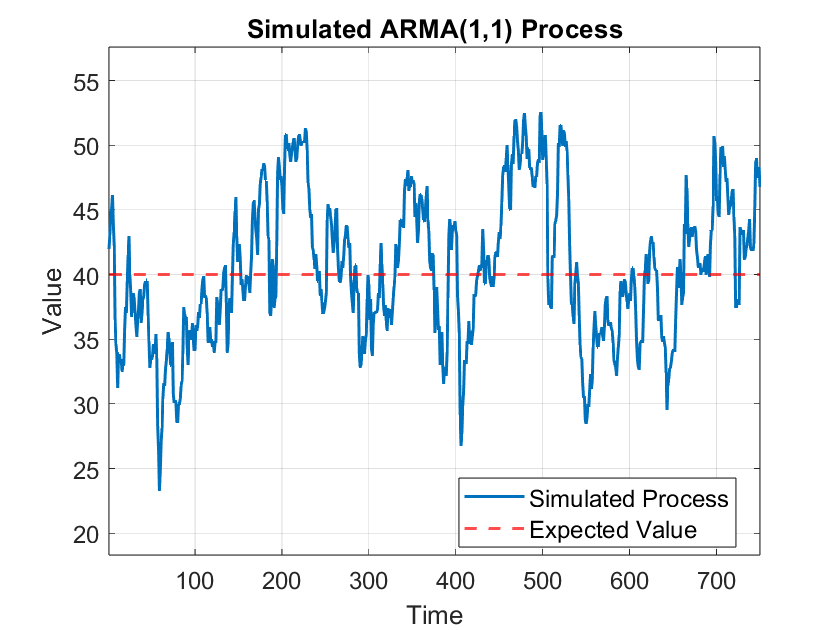
\includegraphics[width=0.8\textwidth]{simulated_arma.png}
    \caption{Simulated ARMA(1,1) Time Series}
    \label{fig:simulated_arma}
\end{figure}

\begin{figure}[H]
     \centering
     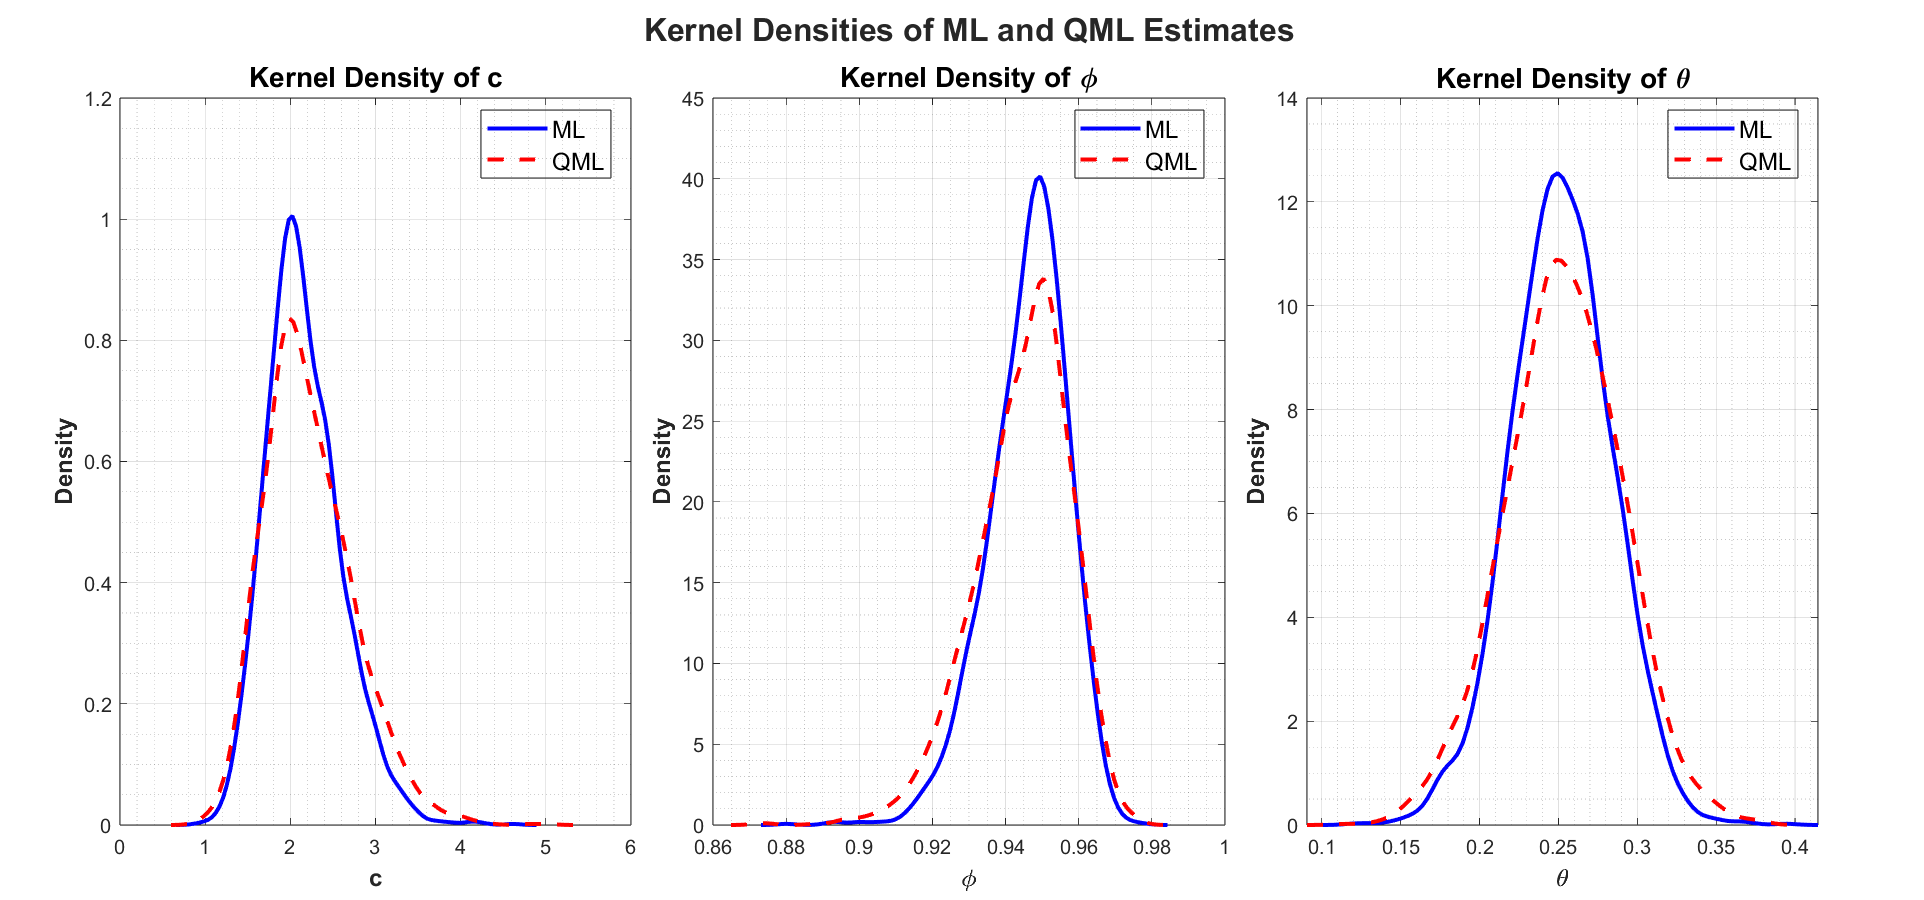
\includegraphics[width=0.8\linewidth]{kde_estimates.png}
     \caption{Kernel Density Plots of Parameter Estimates (ML vs.\ QML)}
     \label{fig:kde_estimates}
\end{figure}

\clearpage
\section{Notes}
\begin{itemize}
    \item The parameter \(\phi\) indicates the persistence in the ARMA(1,1) process.
    \item Interpretation of $t$-tests depends on whether distributional assumptions (e.g., normality) hold.
\end{itemize}

\clearpage
\begin{thebibliography}{9}

\bibitem[Hamilton(1994)]{Hamilton1994}
Hamilton, J.D. (1994).
\textit{Time Series Analysis}.
Princeton University Press.

\bibitem[Hansen(2022)]{Hansen2022}
Hansen, B. (2022).
\textit{Econometrics}.
Princeton University Press.

\bibitem[Hayashi(2000)]{Hayashi2000}
Hayashi, F. (2000).
\textit{Econometrics}.
Princeton University Press.

\end{thebibliography}

\end{document}
